\documentclass[11pt,a4paper]{report}
 \usepackage[francais]{babel}
 \usepackage[utf8]{inputenc}
\usepackage[T1]{fontenc}
\usepackage{graphicx}
\usepackage{caption}
\usepackage{amssymb}
\usepackage{amsmath}
\usepackage{listings}
\usepackage{scrextend}
\usepackage{caption}
\usepackage{xcolor}
\usepackage[toc,page]{appendix}
\usepackage[margin=2 cm]{geometry}
%\usepackage[symbols]{circuitikz}
%\usepackage{tikz}
\lstset{language=R,
basicstyle=\fontfamily{pcr}\selectfont\footnotesize\color{black},
frame = single}
\title{Regression Quantile}

\date{2018}

\begin{document}

%\tableofcontents







\section*{Avantages et inconvénients des Jeux de Synthèse}

Avantages:
\begin{enumerate}
\item On peut générer autant de données que l’on souhaite
\item On peut souvent contrôler, voir jusqu'à supprimer le drift
\item Jeux de données benchmarks référencé dans plusieurs papiers.
\item Pas de traitement préalable
\end{enumerate}

Inconvénients:
\begin{enumerate}
\item Environement contrôlé ne pouvant pas représenter le caractère imprévisible des dérives réelles.
\end{enumerate}
\section*{Jeu de données synthétiques}


\begin{tabular}{ |p{3cm}||p{3cm}|p{3cm}|p{3cm}|p{3cm}|  }

 \hline

 \multicolumn{5}{|c|}{Benchmarks Synthétiques} \\
 \hline
 Nom &Type de drift&Dimension & Drift récurrents & Remarques\\
 \hline 
 AGRAWAL   & Soudain    & 6 numériques, \newline 3 catégoriques &   Non & \\
 Sine 1 &  Soudain & 2 numériques & Oui & \\
 Sine 2 & Soudain & 2 numériques &  Oui & \\
 SINIRREL1 & Soudain & 4 numériques & Oui & Même que Sine1 avec 2 attributs sans impact en +\\
  SINIRREL2 & Soudain & 4 numériques & Oui & Même que Sine2 avec 2 attributs sans impact en +\\
 STAGGER    & Soudain & 3 catégoriques & Adaptable &\\
 Circles		&   Incrémental  & 2 numériques & Adaptable&\\
 MIXED2 &   Incrémental  & 2 numériques, \newline 2 booléens& Oui& \\
 RandomRBF &  Incrémental & $n$ numériques & Non& \\
 LED & & 24 booléens dont 17 impertinents & ?& \\
 Rotating Hyperplane  & Incrémental & $n$ numériques & Adaptable& \\
 Guauss & Incrémental & numériques & Adaptable& \\
 SEA Concept & Incrémental & 3 numériques & Adaptable & \\
 1CDT & Incrémental & 2 numériques & Moyennement  & \\
2CDT & Incrémental& 2 numériques& Moyennement  & \\
1CHT & Incrémental& 2 numériques& Moyennement  &  \\
2CHT & Incrémental& 2 numériques& Moyennement  &   \\
4CR & Incrémental& 2 numériques & Adaptable  &  \\
4CRE-V1& Incrémental & 2 numériques &  Moyennement  & \\
4CRE-V2 & Incrémental& 2 numériques & Moyennement  & \\
5CVT & Incrémental& 2 numériques & Moyennement  & \\
1CSurr & Incrémental& 2 numériques& Moyennement  & \\
4CE1CF & Incrémental& 2 numériques & Adaptable  &  \\
UG-2C-2D & Incrémental& 2 numériques& Moyennement  &  \\
MG-2C-2D & Incrémental& 2 numériques& Moyennement  & \\
FG-2C-2D & Incrémental& 2 numériques& Moyennement  & \\
UG-2C-3D & Incrémental& 3 numériques& Moyennement  &  \\
UG-2C-5D & Incrémental& 5 numériques & Moyennement  & \\
GEARS-2C-2D & Incrémental & 2 numériques& Adaptable  & \\
 \hline
\end{tabular}




Certains jeux de données ont été générés et sont figés. Cependant, on pourrait très bien les regénérer afin de fabriquer une dérive récurrentes. On peut aussi modifier à notre guise les jeux de données pour les rendre aussi long que l'on souhaite.

Voici un petit descriptif des jeux de données.

\begin{itemize}
\item Sine 1: It consists of two attributes x and y uniformly distributed in [0, 1]. The classification function is y = sin(x). Instances are classified as positive if they are under the curve; otherwise they are classified as negative. At a drift point, the class labels are reversed.

\item Sine 2: It holds two attributes of x and y which are uniformly distributed in $[0, 1]$. The classification function is $0.5 + 0.3 * sin(3\pi x)$. Instances under the curve are classified as positive while the other instances are classified as negative. At a drift point, the classification scheme is inverted. 

\item Stagger: This dataset contains three nominal attributes, namely size $= [small, medium, large], color=[red, green]$, and shape=$[circular, non-circular]$. Before the first drift point, instances are labeled positive if $[color = red]$ and $[size = small]$. After this point and before the second drift, instances are classified positive if$ [color = green] v [shape = circular]$, and finally after this second drift point, instances are classified positive only if $[size = medium] ou [size = large]$.

\item Circles: It has two attributes x and y that are distributed in [0, 1]. The function of circle $<(x_c,y_c), r_c> is (x - x_c)^2 + (y - y_c)^2 = r_c^2$ where $(x_c, y_c)$ is its center and $r_c$ is the radius. Four circles of $<(0.2, 0.5), 0.15>, <(0.4, 0.5), 0.2>, <(0.6, 0.5), 0.25>,$ and $<(0.8, 0.5), 0.3>$ classify instances in order. Instances inside the circle are classified as positive. A drift happens whenever the classification function, i.e. circle function, changes.

\item MIXED2 (3M): The dataset has two boolean attributes (v, w) and two continuous attributes (x, y) from [0,1]. The examples are classifiedas positive if at least two of the three following conditions are satisfied: $v, w, y < 0.5 + 0.3 * sin(3\pi x)$. After each change, the classification is reversed. Noise is introduced by switching the labels of 10\% of the examples

\item RandomRBF: Uses n centroids with their centers, labels and weights randomly defined, and a Gaussian distribution to determine the values of m attributes. A concept drift is simulated by changing the number and positions of the centroids. This dataset has six classes, 40 attributes and 50 centroids. 

\item LED: Represents the problem of predicting the digit shown by a seven-segment LED display. It has 24 categorical attributes, 17 of which are irrelevant, and a categorical class, with ten possible values. Also, each attribute has a 10\% probability of being inverted (noise). Concept drifts are simulated by changing the position of the relevant attributes. 


\item Rotating Hyperplane : The orientation and position of a hyperplane in d-dimensional space is changed to produce concept drift

\item GAUSS (2G) The examples are labeled according to two different but overlapped Gaussian, $\mathcal{N}([0,0],1])$ and $\mathcal{N}([2,0],4)$. The overlappingcan be considered as noise. After each change, the classification is reversed.

\item Sea Concept: The Sea Concepts dataset is an artificial adapted for novelty detection and originally proposed by Street and Kim (2001). It consists of 60,000 instances with three attributes of which only two are relevant. The two class decision boundary is given by f1 + f2 = b, where f1, f2 are the two relevant features and b is a predefined threshold. Abrupt drift is simulated with four different concepts by changing the value of b. The dataset contains 10\% of noise. 

\end{itemize}



\newpage



https://sites.google.com/site/nonstationaryarchive/datasets

\begin{figure}[h]
    \centering
    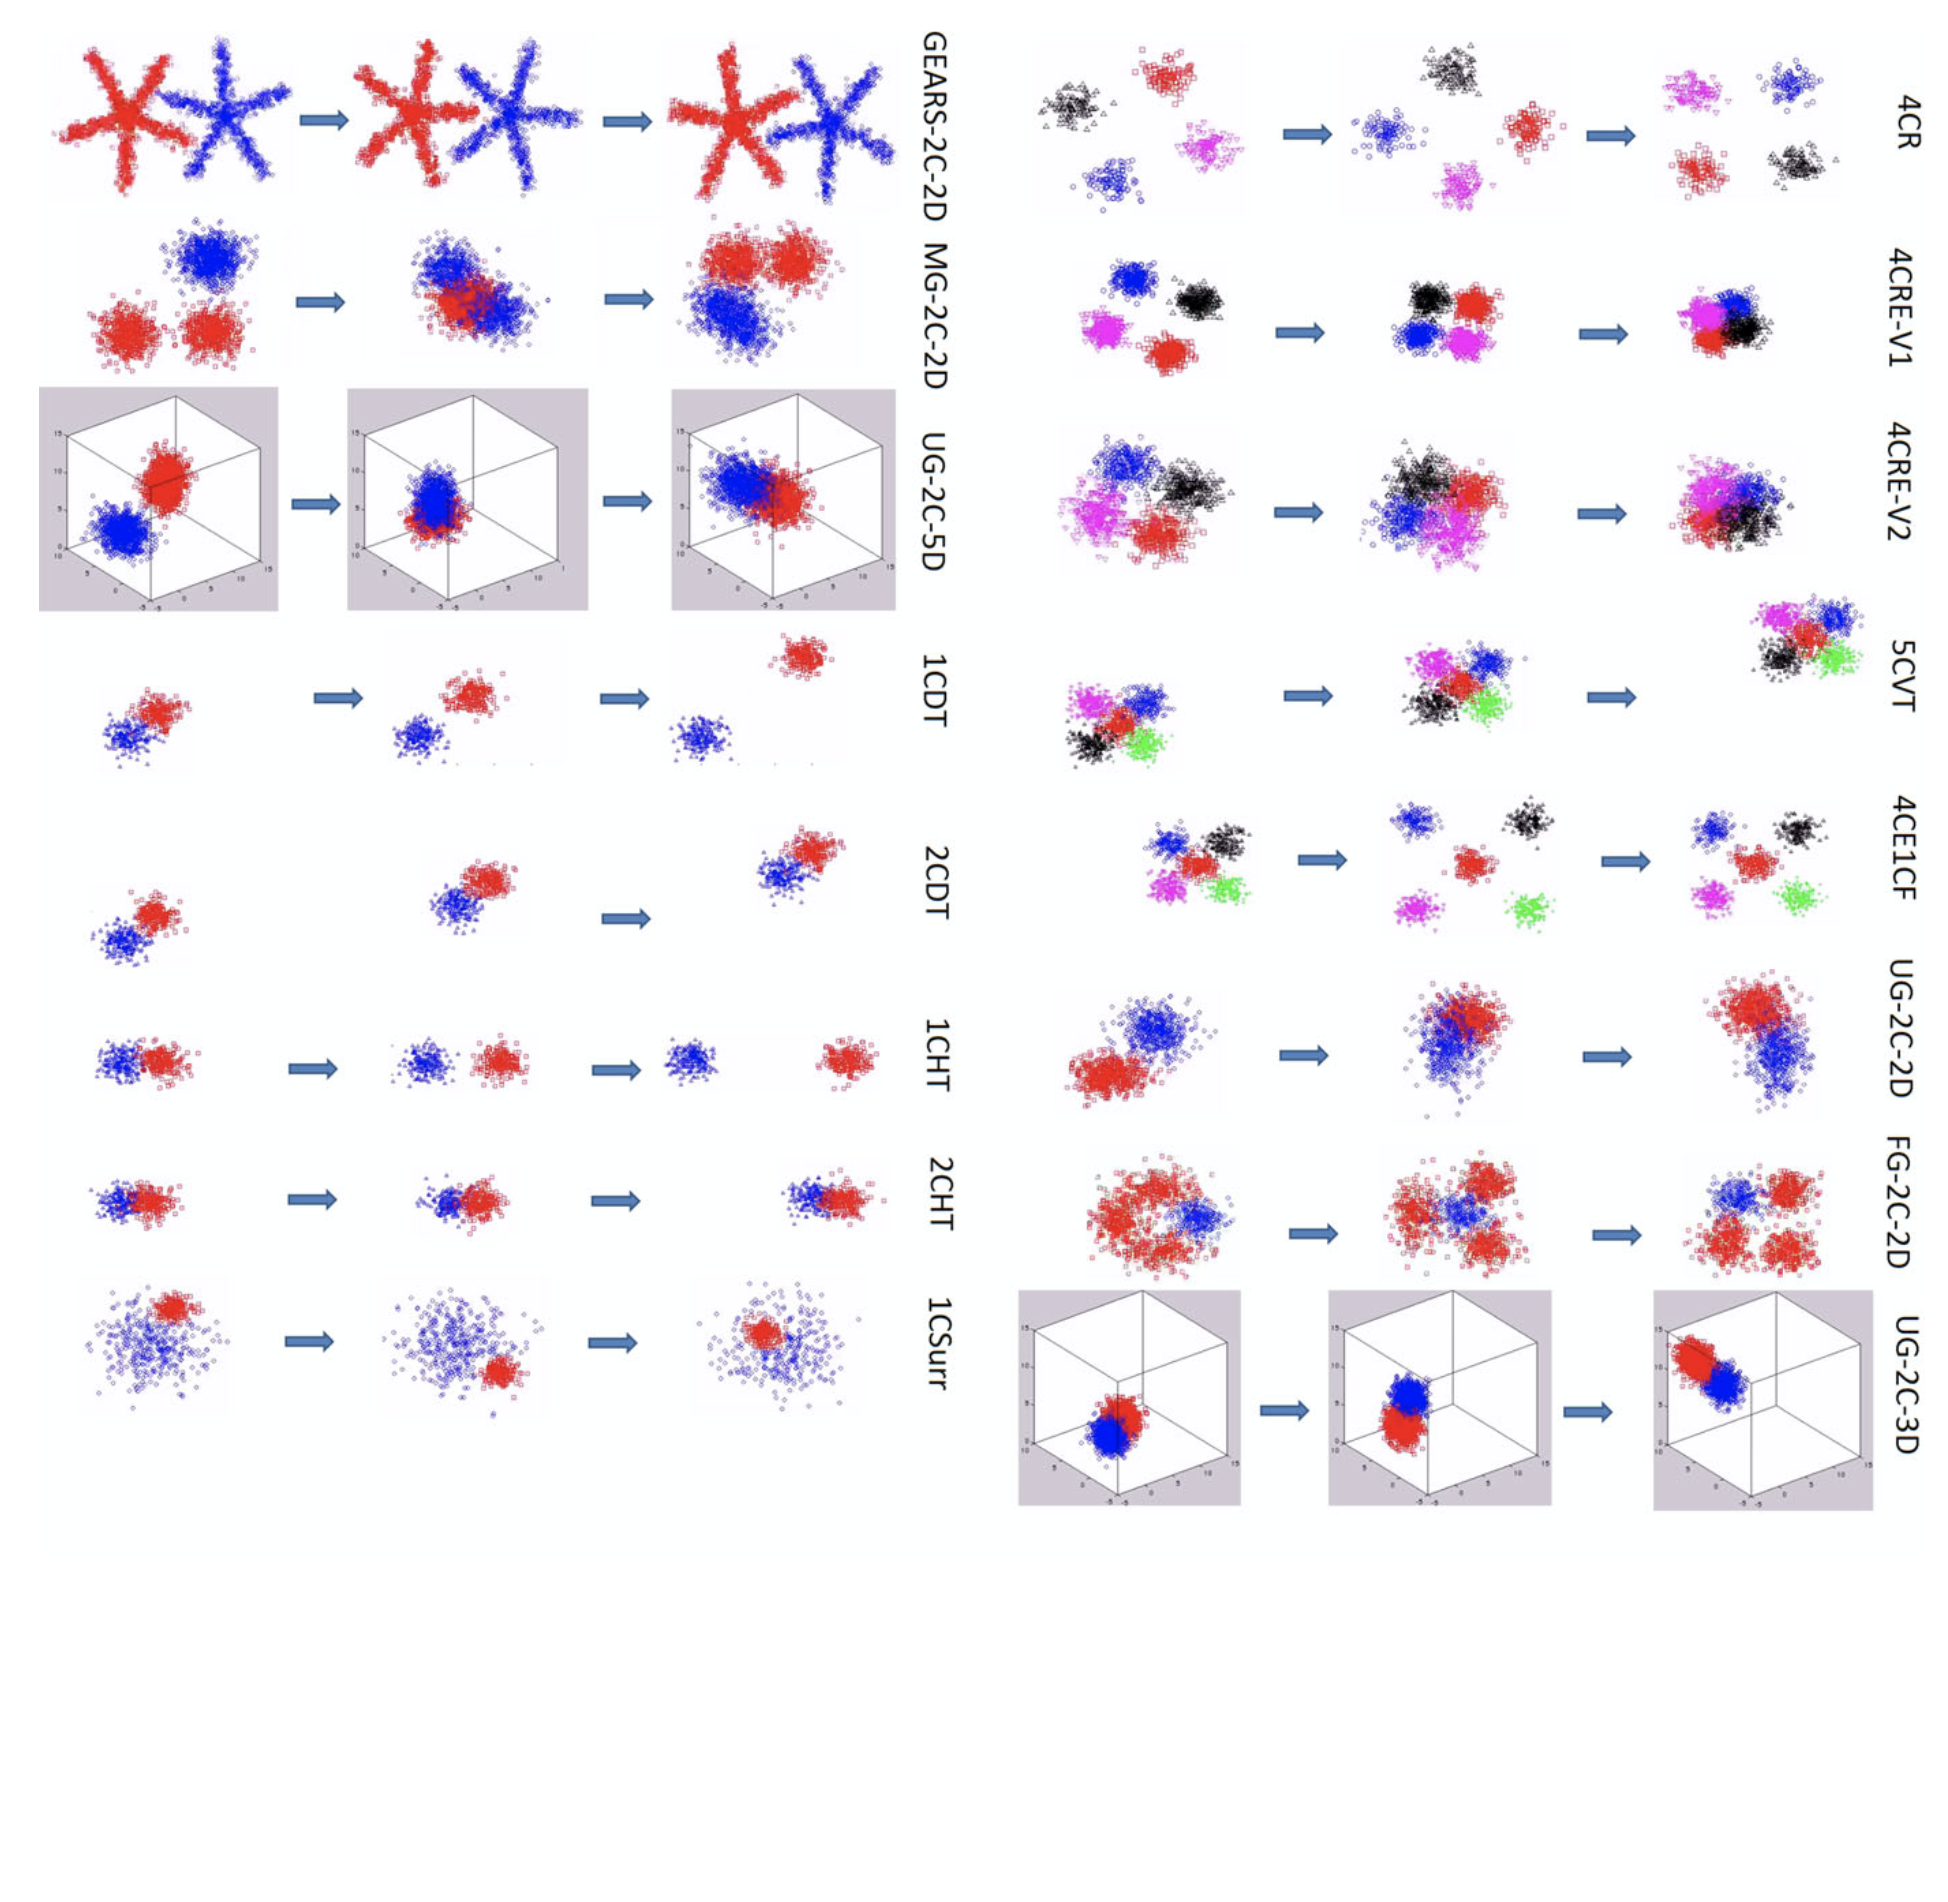
\includegraphics[width=\textwidth]{datasets_synthetiques}
    \caption{Visualisation de l'évolution d'une partie jeux de données}
\end{figure}



\chapter*{Jeu de données réels}

\begin{itemize}

\item Elec: Le jeu de donné réel le plus couramment utilisé dans l'évaluation de solution de détection de dérive est le jeu de donnée des prix d’électricité. Il contient deux variables pour le jours et l’heure, puis 4 variables pour décrire le prix et la demande.
L'avouvent cité.
Inconvénients : Peu de variables, nombre d’observations fini.


\item Covertype: contains 30 m * 30 m cells of data from US Forest Service (USFS) Region 2. It has 581,012 instances and 54 attributes, both numeric and categorical, and the goal is to predict the forest cover type. The version we used was sorted by the elevation attribute, which induces a natural gradual concept drift on the class distribution. This occurs because, depending on the elevation, some types of vegetation disappear while others start to appear. 

\item Airlines : is a binary dataset composed of 539,383 instances. The goal is to predict whether flights are delayed or not, based on a set of flight information: name of the company, departure time, flight number, duration, airports of origin and destination, and day of the week. 

\item Emailing list dataset : Dataset traduisant un flux d’emails triés par des utilisateurs en email intéressant ou non, où les goûts des utilisateurs changent (oscillent) avec le temps. (Concept drift récurrent)

\item Spam filterig dataset : Dataset de mail par ordre chronologique dont sont dérivés 500 variables. Les emails sont identifiés comme spam où non. Les profils type des spam change avec le temps ce qui en fait problème de drift conceptuel progressif.

\item The Weather dataset is originally proposed and described in Elwell and Polikar (2011) in order to predict whether it is going to rain on a certain day or not. The dataset contains 18159 instances with an imbalance towards no rain (69\%). Each sample is described with eight weather-related features such as temperature, pressure, wind speed etc. 

\item Covtype dataset is introduced in Blackard and Dean (1999) and often used as a benchmark for drift algorithms. It assigns cartographic variables such as elevation, slope, soil type, etc. to different forest cover types. Only forests with minimal human- caused disturbances were used, so that resulting forest cover types are more a result of ecological processes. 

\item Outdoor: (Losing et al. 2015) is obtained from images recorded by a mobile in a garden environment. Images contain 40 different objects, each approached ten times under varying lighting conditions affecting the color based representation. Each approach consists of 10 images and is represented in temporal order within the dataset. 

\item The Rialto dataset: (Losing et al. 2016) consists of images of colorful buildings next to the famous Rialto bridge in Venice, encoded in a normalized 27-dimensional RGB histogram. Images are obtained from time-lapse videos captured by a webcam with fixed position. The recordings cover 20 consecutive days. Continuously changing weather and lighting conditions affect the representation. 

\item The Keystroke dataset (described in Souza et al. (2015)) is from a real-world appli- cation related to keystroke dynamics for recognizing users by their typing rhythm, where user profiles evolve incrementally over time. 

\item The Usenet dataset is a text dataset inspired by Katakis et al. (2010) and processed for novelty detection. It consists of a simulation of news filtering with concept drift related to the change of interest of a user over time. A user can decide to unsubscribe from news groups that he is not interested in and subscribe for new ones that he becomes interested in, and the previously interesting topics become out of his main interest. 

\end{itemize}













\end{document}